\documentclass[12pt]{article}
\usepackage[utf8]{inputenc}
\usepackage{amsmath}
\usepackage[T1]{fontenc}

\title{ECE 3413 Lab 08\\*DC Motor Model for Open-loop Control in MATLAB Simulink}
\author{Leomar Dur\'an}
\date{${12}^{\text{th}}$ April 2023}

\usepackage[natbib,style=apa6]{biblatex}
\addbibresource{main.bib}
\defbibheading{bibliography}[\refname]{%
  \section*{\centering #1}%
}%

\usepackage{hyperref}

\usepackage{cancel}
\usepackage[per-mode=symbol]{siunitx}
\newcommand*\siexpr[2][]{\SI[parse-numbers=false,#1]{#2}}%
\usepackage{xfrac}
\usepackage{amssymb}
\newcommand*\transpose{\mathsf{T}}

\usepackage{mathtools}%
\DeclarePairedDelimiter\brao()%
\DeclarePairedDelimiter\brac[]%
\DeclarePairedDelimiter\braco[)%
\DeclarePairedDelimiter\braoo][%
\DeclarePairedDelimiter\Brac\{\}%
\DeclarePairedDelimiter\abs||
\DeclarePairedDelimiter\norm\lVert\rVert%
\DeclarePairedDelimiter\piecefn\{.
\DeclarePairedDelimiter\evalat.|

\usepackage{lib/nonfloatenvirons}
\usepackage{booktabs}
\newcommand\ra[1]{\renewcommand*\arraystretch{#1}}
\ra{1.25}

\usepackage{minted}
\newcommand\matlab{matlab}

\usepackage{adjustbox}
\newcommand{\setprime}[2][1]{%
    {#2}^{%
        \raisebox{1pt}{%
            \scalebox{0.5}{%
                \itshape\sffamily\uppercase%
                \expandafter{%
                    \romannumeral#1%
                }%
            }%
        }
    }%
}%
\newcommand*\mcadj[7]%
% {#columns}{col spec}{rotation}{adjust spec}
% {before rotated text}{rotated text}{after rotated text}
{%
    \multicolumn{#1}{#2}{%
        \rlap{%
            #5\adjustbox{rotate=#3,#4}{#6}~#7%
        }%
    }%
}

\usepackage{pdfpages}
\usepackage{standalone}
\usepackage{matlab}

\usepackage[skip=\baselineskip,indent=0pt]{parskip}
\setlength\parindent{0pt}

\usepackage[shortlabels]{enumitem}

\def\hr{{\par\noindent\rule{\textwidth}{0.4pt}}}

\begin{document}

\maketitle
\newpage

\section{Introduction}

This is a two week lab.
Included are both week \texttt\#01 and week \texttt\#02.

The purpose of this lab in week 01 is to analyze a transfer function
and a set of modifications to that transfer function,
whether that be scaling the components of the poles, the natural frequency or adding poles.

This allows us to form relations between these parameters and the characteristics that we expect from a transfer function such as the transient response.

Not only can we estimate the effects that a modification will have on a transfer function, but we can use these relations to find new transfer functions just as one would pick components to have specific effects on a circuit.

In week 02, we also explore the damping of systems and feedback.

\section{Procedure}\label{sec:procedure}

\subsection{Task 1 -- Varying the gains}\label{ssc:vary gains}



\begin{figure}
    \centering
    \includegraphics[width=.8\linewidth]{img/lab06-0000-negative_feedback_system.png}
    \caption{A parameterized negative feedback system.}
    \label{fig:negative feed back system}
\end{figure}

Given the negative feedback system in Fig.~\ref{fig:negative feed back system}
with
\begin{equation}
    \piecefn*{
        \begin{array}{@{}l@{}}
            \displaystyle
            G\brao*s = \frac{K}{s\brao{s + 2}^2},\\*
            H\brao*s = 1,
        \end{array}
    }
\end{equation}

the equivalent transfer function is
\begin{equation}
    \begin{aligned}
        \brao*{\frac{C}{R}}\brao*s
            &{}= \frac{G\brao*s}{1 + \brao*{GH}\brao*s}
    \\*
            &{}= \frac{1}{\displaystyle\sfrac1{G\brao*s} + H\brao*s}
    \\*
            &{}= \frac{1}{\displaystyle\brao*{\frac{s\brao*{s + 2}^2}K} + \brao*1} \times \frac{K}K
    \\*
            &{}= \frac{K}{s\brao*{s + 2}^2 + K}
    \\*
            &{}= \frac{K}{s^3 + 4s^2 + 4s + K}.
    \\*
    \end{aligned}
\end{equation}

\subsection{Task 2 -- Overdamped and underdamped systems}

\subsubsection{Finding an overdamped system}\label{sss:overdamped procedure}

First we must find the critical damping point.

This is found by first finding the characteristic equation, which is the denominator of the transfer function fix at $0$.
\begin{equation}
    s^3 + 4s^2 + 4s + K = 0.
\end{equation}

Let's generalize this characteristic equation with $p, q \in \mathbb{R}$ to
\begin{equation}
    s^3 + ps^2 + qs + K = 0.
\end{equation}

Then we solve for $K$.
\begin{equation}
    K = -s^3 - ps^2 - qs.
%    K = -s^3 - 4s^2 - 4s.
\end{equation}

We next find the fix the derivative of $K$ at $0$.
\begin{equation}
    0 = \evalat*{\frac{dK}{ds}}_{s=s_0} = -3s^2 - 2ps - q,
%   \evalat*{\frac{dK}{ds}}_{s=s_0} = -3s^2 - 8s - 4,
\end{equation}
and solve for $s_0$.
\begin{equation}
    s_{1,2} = %\brac*{\begin{matrix}
        \frac{+2p}{-6} \pm \frac{\sqrt{p^2 - 3q}}{-3}%
%        -2 \\* -\sfrac23
    %\end{matrix}}
    .
\end{equation}

After this point, the equation gets very complex and we will need to know the value of $K$ anyway. So let's substitute our coefficients $p = 4, q = 4$ into
\begin{equation}
    s_{1,2} = \brac*{\begin{matrix}
        -\sfrac63 \\* -\sfrac23
    \end{matrix}}%
    ,
\end{equation}
and solve for $K \not= 0$ again. This gives the critical damping point

\begin{equation}\label{eq:critical damping point}
    \Brac*{ K \middle| \brao*{K = \evalat*{\brao*{-s^3 - 4s^2 - 4s}}_{s \in s_{1,2}}}} \setminus \Brac0 = \Brac{\sfrac{32}{27}} \ni K_{\zeta=1}.
\end{equation}

Thus, if $K = \sfrac{32}{27} = K_{\zeta=1}$, then the system is critically damped. However, if $K < \sfrac{32}{27} = K_{\zeta=1}$, then the system is overdamped for overdamped systems.

Let's pick two gains $K = \sfrac{32}{27} - \SI4\percent = \sfrac{3072}{2700}$ and $K = \sfrac{32}{27} - \SI{10}\percent = \sfrac{2880}{2700}$.

\subsubsection{Finding an underdamped system}\label{sss:underdamped procedure}

We have a lower limit for a possibly underdamped system given above as $K_{\zeta=1}$.

To find the upper limit, we will need to use the Routh--Hurwitz criterion.

We start by making a table with one more rows as the degree of the denominator of the transfer function.
We populate the top two rows by alternatingly filling them with the coefficients of the denominator in order of descending degree.
If the last spot is empty, we fill it with $0$. We also add a last $0$ column.

\begin{table}[h]
    \centering
    \[
        \begin{array}{@{}*4r@{}}
            s^3: &                          1 & 4 & 0 \\*
            s^2: &                          4 & K & 0 \\*
%            s^1: &                          0 & 0 & 0 \\*
%            s^0: &                          0 & 0 & 0 \\*
        \end{array}
    \]
    \caption{First two rows of the Routh--Hurwitz table.}
    \label{tab:rh table 1st 2 rows}
\end{table}

Next we populate the remaining rows by filling each cell up to and including the penultimate of each column with the determinant of the $2\times2$ matrix formed by the first column and the column succeeding this column for the previous two rows, all divided by the first cell of the previous row.

For example, the first cell of row $s^1$ gets
$
    \dfrac14\abs*{
        \begin{matrix} 1 & 4 \\* 4 & K\end{matrix}
    } = 4 - K/4,
$

and the second cell of the same row gets
$
    \dfrac14\abs*{
        \begin{matrix} 1 & 0 \\* 4 & 0\end{matrix}
    } = 0.
$

The final column always gets $0$, resulting in the table.

\begin{table}[h]
    \centering
    \[
        \begin{array}{@{}*4r@{}}
            s^3: &                          1 & 4 & 0 \\*
            s^2: &                          4 & K & 0 \\*
            s^1: &                    4 - K/4 & 0 & 0 \\*
            s^0: & (K*(K - 16))/(4*(K/4 - 4)) & 0 & 0 \\*
        \end{array}
    \]
    \caption{The complete Routh--Hurwitz table.}
    \label{tab:rh table complete}
\end{table}

Next, we find the first row and corresponding $K$-values for which $\exists K$ s.t. the entire row is $0$.
The $K$-value of this first \textsc{zero} row is at the marginal stability point.

In row $s^1$, the value $K = 16$ gives $4 - K/4 = 4 - \brao*{16}/4 = 0$ thus giving the row $\begin{matrix}s^1: & 0 & 0 & 0\end{matrix}$.
Therefore the marginal stability point
\begin{equation}\label{eq:marginal stability point}
    K_{a=0} = 16.
\end{equation}

From the marginal stability point, we have that $K = 16 = K_{a=0}$ produces a system that is marginally stable and undamped, and we have that $K > 16 = K_{a=0}$ produces an unstable system.

Now if $K \in \braoo{\sfrac{32}{27}, \sfrac{432}{27}} = \braoo{K_{\zeta=1}, K_{a=0}}$, then the system is underdamped.

\subsection{Task 3 -- Critically damped system}

By fixing the derivative $\frac{dK}{ds} = 0$ in sub-subsection~\ref{sss:overdamped procedure}%
, we found \eqref{eq:critical damping point},
which gives us gain $K_{\zeta=1} = \sfrac{32}{27}$
at the critical damping point, which produces a critically damped system.

\subsection{Task 4 -- Marginally stable system}

Through the Routh--Hurwitz criterion in sub-subsection~\ref{sss:underdamped procedure}%
, we found \eqref{eq:marginal stability point},
which gives us gain $K_{a=0} = 16$
at the marginal stability point, which produces a marginally stable undamped system.

Furthermore, from Table~\ref{tab:rh table complete}, in the $s^2$ row, we have $4s_n^2 + K = 0$. Since $K = 16$ at the marginal stability point, then the complex natural frequency
\begin{equation}
    s_n = 0 \pm j2 = \sigma_n \pm j\omega_n.
\end{equation}

Thus the frequency of oscillation $\omega_n = \SI{2}{\radian\per\second}$.

\section{Results}

\subsection{Task 1 -- Negative feedback system-equivalent transfer function}

In the \nameref{sec:procedure} subsection~\ref{ssc:negative feedback equivalent}, we algebraically found that the system that we are analyzing is equivalent to the transfer function

\begin{equation}
    \brao*{\frac{C}{R}}\brao*s = \frac{K}{s^3 + 4s^2 + 4s + K}.
\end{equation}

\subsection{Task 2 -- Overdamped and underdamped systems}

\subsubsection{Overdamped systems}\label{sss:overdamped results}

\begin{figure}
    \centering
    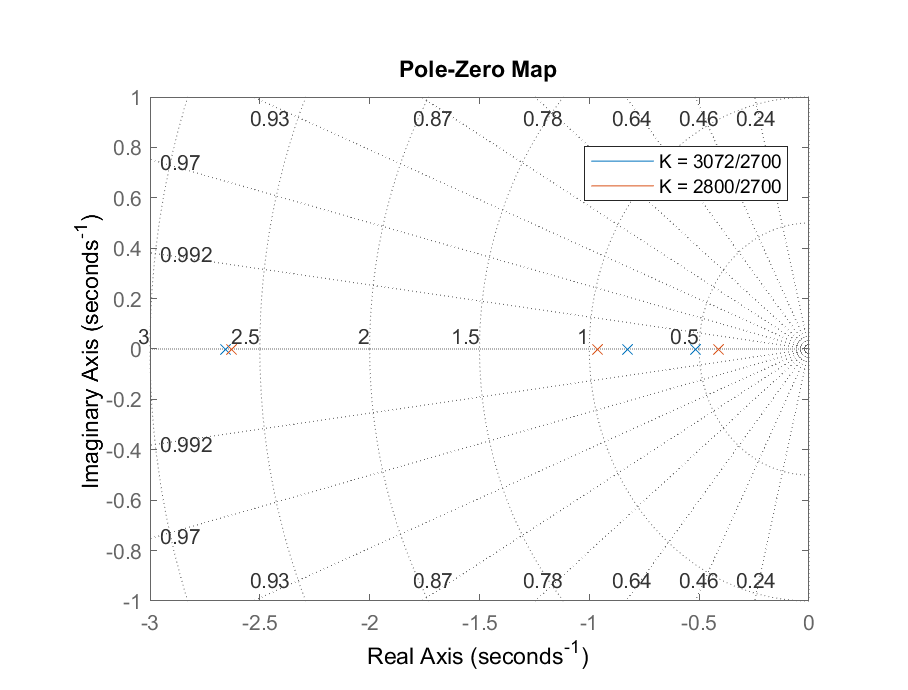
\includegraphics[width=\linewidth]{img/task02_01_overdamped_pzmap.eps}
    \caption{Pole-zero map of the overdamped system.}
    \label{fig:overdamped pzmap}
\end{figure}

In sub-subsection~\ref{sss:overdamped procedure} we found%
, by fixing the derivative $\frac{dK}{ds} = 0$,
that overdamped systems of this family of transfer functions have gain $K < \sfrac{32}{27}$.
so let's pick two gains $K_1 = \sfrac{32}{27} - \SI4\percent = \sfrac{3072}{2700}$ and $K_2 = \sfrac{32}{27} - \SI{10}\percent = \sfrac{2880}{2700}$.
We can see the poles produced by bother example gains in \ref{fig:overdamped pzmap}.

\begin{enumerate}
    \item 
        The cubic system with gain $\sfrac{3072}{2700}$ produces poles $s_{1,2,3} = -2.6547,$ $-0.8272,$ $-0.5181$.
    \item
        The cubic system with gain $\sfrac{2880}{2700}$ produces poles $s_{1,2,3} = -2.6361,$ $-0.9277,$ $-0.4362$.
\end{enumerate}

From inspection, these a unique triplet of poles are all negative real poles.

\subsubsection{Underdamped system}

\begin{figure}
    \centering
    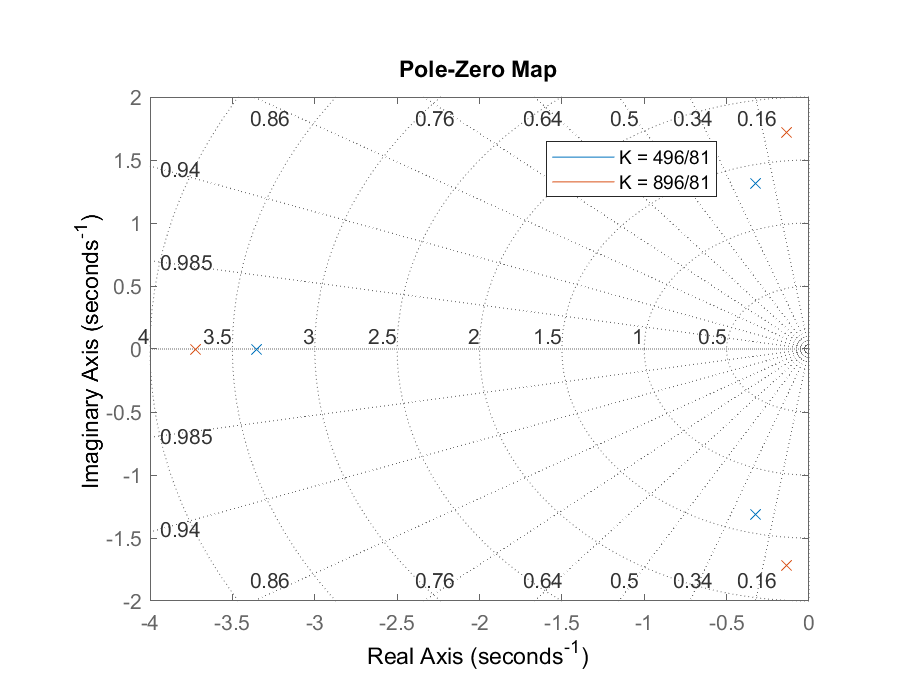
\includegraphics[width=\linewidth]{img/task02_02_underdamped_pzmap.eps}
    \caption{Pole-zero map of the underdamped system.}
    \label{fig:underdamped pzmap}
\end{figure}

In sub-subsection~\ref{sss:underdamped procedure} we found%
, by fixing the derivative $\frac{dK}{ds} = 0$ and through the Routh--Hurwitz criterion,
that underdamped systems of this family of transfer functions have gain $K \in \braoo{\sfrac{32}{27}, \sfrac{432}{27}}$.
so let's pick two gains $K_1 = E\brac*{\brao*{\sfrac{32}{27}}^2, \brao*{\sfrac{432}{27}}^1} = \sfrac{496}{81}$ and $K_2 = E\brac*{\brao*{\sfrac{32}{27}}^1, \brao*{\sfrac{432}{27}}^2} = \sfrac{896}{81}$.
We can see the poles produced by bother example gains in \ref{fig:underdamped pzmap}.

\begin{enumerate}
    \item 
        The cubic system with gain $\sfrac{496}{81}$ produces poles $s_{1,2,3} = -3.3517,$ $-0.3242 \pm j1.3122$.
    \item
        The cubic system with gain $\sfrac{896}{81}$ produces poles $s_{1,2,3} = -3.7236,$ $-0.1382 \pm j1.7180$.
\end{enumerate}

From inspection, these poles are complex numbers with negative real part. There must be at least one pair of complex conjugates and the other pole is purely real.

\subsection{Task 3 -- Systems with gains in the inflection points}

\begin{figure}
    \centering
    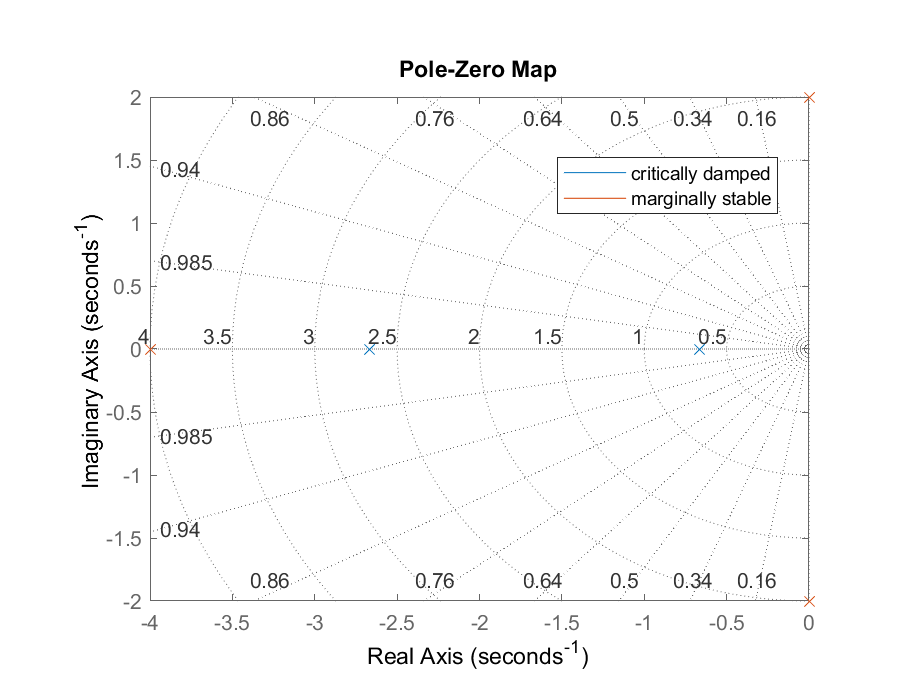
\includegraphics[width=\linewidth]{img/task02_03_04_inflection_pzmap.eps}
    \caption{Pole-zero map of the critically damped and marginally stable systems.}
    \label{fig:inflection points pzmap}
\end{figure}

\subsubsection{Critically damped system}

In sub-subsection~\ref{sss:overdamped procedure}, we found the gain at the critical damping point, $K_{\zeta=1} = \sfrac{32}{27}$, which produces a critically damped system.
The cubic system with this gain produces poles $s_{1,2,3} = -\sfrac83,$ $-\sfrac23,$ $-\sfrac23$.

Unlike the poles of overdamped systems in sub-subsection~\ref{sss:overdamped results},
the triplet of poles of the critically damped system contains a double root at $s = -\sfrac23$.

\subsubsection{Marginally stable system}

In sub-subsection~\ref{sss:underdamped procedure}, we found the gain at the marginal stability point, $K_{a=0} = 16$, which produces a marginally stable system.
The cublic system with this gain produces poles $s_{1,2,3} = -12,$ $\pm j6$.

The marginally stable system produces $1$ real pole and a pair of purely imaginary conjugates (which categorically have \textsc{zero} real part).



\section{Discussion}

\paragraph{For week 01}

In this lab, we learned that manipulating the real and imaginary parts of the poles will effect their $x$- and $y$-components respectively, and that manipulating the natural frequency will effect the poles' magnitudes.

Regarding this, I learned that graphing in the polar co\"ordinate system is not as well supported by Matlab as the Cartesian co\"ordinate system.
There is a \mintinline\matlab{polarplot} function.
However it does not support multiple plots and cannot be combined with a plot in Cartesian.
Because of this, going forward, I will use \mintinline\matlab{pzmap} instead;
and if I need to use the more primitive facilities of polar co\"ordinate system,
then I will have to prefer to find an alternative system such as Python.


This lab also gave us the opportunity to test the hypothesis that a positive real pole will always be result in an unstable transfer function, whereas a transfer function where all poles only have non-positive real part will be stable.
Additionally, we have learned that the poles with real part closest to $0$ dominate.
It is also a good time to remember that a pole that has $5\times$ the real part $-\zeta\omega_n$ of another pole
will have very little significant effect in comparison.
This former pole is $5\tau$ away from the latter pole.

Now we can see that the rise time has no direct relationship with the roots or the natural frequency.
Because of this, we had to use the Matlab equation solver to find the appropriate times at $\SI{10}\percent$ and $\SI{90}\percent$ final output,
and from this calculate the rise times.

From Table~\ref{tab:rise time changing poles}, we can confirm no obvious relation for the components of the pole. However, there seems to be a scaling effect to the natural frequency. Let's investigate further.

\begin{figure}
    \centering
    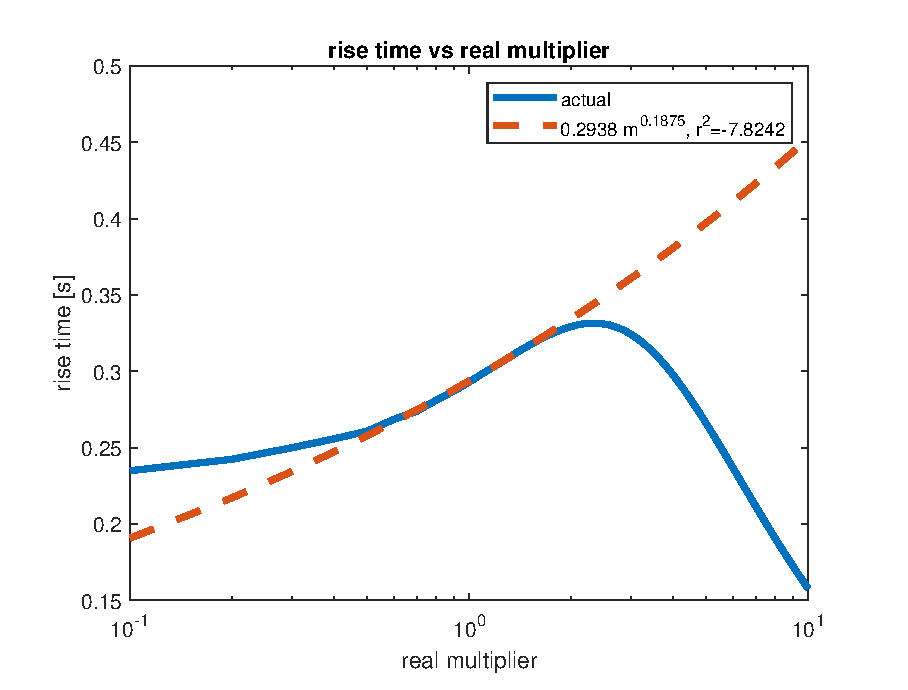
\includegraphics[width=\linewidth]{img/part01_rise_time_vs_real.eps}
    \caption{Plot in a semi-log scale on the $x$-axis
    showing the effect of multiplying the real component of the poles on the rise time and log-log linear regression.}
    \label{fig:rise time vs real}
\end{figure}

The script in Appendix subsection~\ref{sap:rise time vs parameters}
plots the rise time vs the parameters that we have investigated
in a semi-log scale on the $x$-axis
from the reciprocal of the modification to the modification.
(For the imaginary part, this is the reverse because the modification was scaling by $\sfrac12$.)
A log-log linear regression is taken from these, and then the entire plot is scaled by $5$ on each side
to allow for scaling.

This produces Fig.~\ref{fig:rise time vs real}, \ref{fig:rise time vs imag} and \ref{fig:rise time vs wn}.

\paragraph{Note that} since the Matlab equation solver is time expensive and each plot will use $100$ samples, we use the Matlab \mintinline\matlab{stepinfo} function to find the rise time, albeit it does not the bounds of the rise time.

\begin{figure}
    \centering
    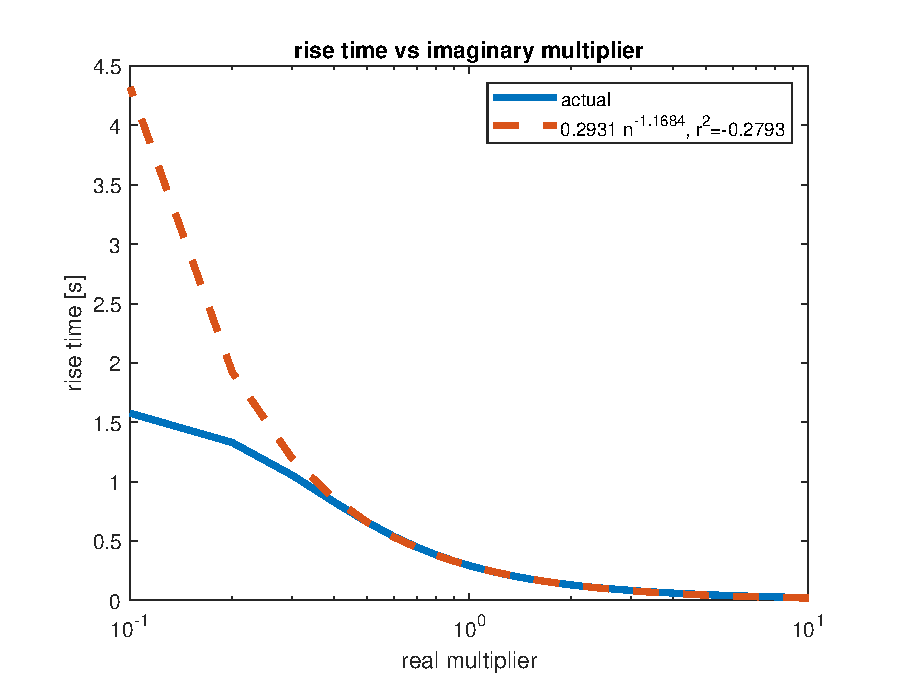
\includegraphics[width=\linewidth]{img/part01_rise_time_vs_imag.eps}
    \caption{Plot in a semi-log scale on the $x$-axis
    showing the effect of multiplying the imaginary component of the poles on the rise time and log-log linear regression.}
    \label{fig:rise time vs imag}
\end{figure}

Now, the coefficients in $\brac{\begin{matrix}0.2938 & 0.2931 & 0.2930\end{matrix}}$ represent the rise time of the original transfer function,
which we found to be \SI{0.292698}\second in sub-subsection~\ref{sss:evaluations}.
These values represent that rise time with deviation $\num{0.00085651}$.

For modifying the real component, the linear regression
(in Fig.~\ref{fig:rise time vs real})
was only successful locally at $\brac{0.3, 2.3}$ with $r^2 = \num{0.956348}$.
Thus, there does not seem to be a relation between the real component and rise time.

\begin{figure}
    \centering
    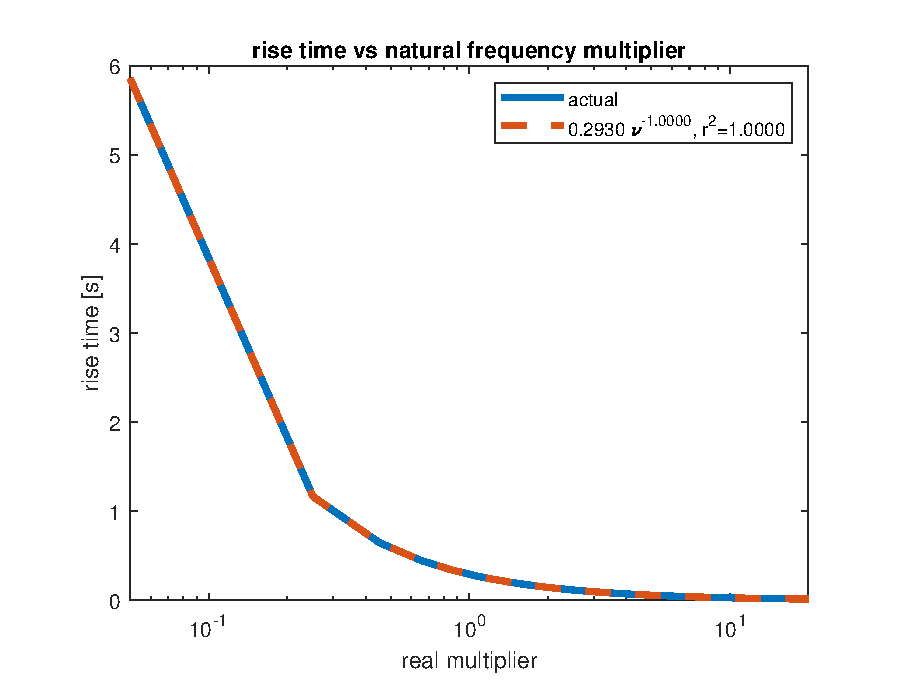
\includegraphics[width=\linewidth]{img/part01_rise_time_vs_wn.eps}
    \caption{Plot in a semi-log scale on the $x$-axis
    showing the effect of multiplying the natural frequency on the rise time and log-log linear regression.}
    \label{fig:rise time vs wn}
\end{figure}

For modifying the imaginary component, the linear regression
(in Fig.~\ref{fig:rise time vs imag})
is much better, having $r^2 = 0.991558$ in $\brac{0.3, 9.8}$.
I predict that after $n = 0.3$, the effect of multiplying the imaginary part by imaginary part of the pole by $n$ will result in a division of the rise time by $n^{1.1684}$.
In fact, taking the original rise time \SI{0.292698}\second and dividing by $\brao*{\sfrac12}^1.1684$ gives $\SI{0.657874}\second$.
The calculated value for the rise time halving the imaginary part of the pole was $\SI{0.658607}\second$.
That's a rate of error of $\SI{-0.111295}\percent$.
Interestingly since the modification was to half the imaginary part, this prediction may not be so useful.

Earlier, we speculated that modifying the natural frequency uniformly moves the range of the rise time.
In Fig.~\ref{fig:rise time vs wn}, we find an $r^2 = 1.0000$ from $\brao{0.05, 19.3955}$.
This appears to be an exact match!
We can predict that multiplying the natural frequency by $\nu$ will result in dividing the rise time by $\nu$.
Now
\begin{equation}
    \frac{T_r}\nu = \frac{\SI{0.292698}\second}4 = \SI{0.0731745}\second \approx \SI{0.073175}\second = \setprime[3]{T}_r
\end{equation}
with a negligible $\SI{-6.83293e-6}{\second^0}$ rate of error.

Moreover, it the natural frequency
scales the time domain
of a transfer function.
Earlier we saw that changing the natural frequency $\setprime\omega_n = \nu\omega_n$ results in
new peak time $\setprime{T}_p = \sfrac{T_p}\nu$ and
new settling time $\setprime{T}_s = \sfrac{T_s}\nu$,
and now we have the relation $\setprime{T}_r = \sfrac{T_r}\nu$
as well as the bounds $\setprime{t}_{.9f} = \sfrac{t_{.9f}}\nu,\ \setprime{t}_{.1f} = \sfrac{t_{.1f}}\nu$
from Table~\ref{tab:rise time changing poles}.
In the case of overshoot, it makes sense that this would not be affected
as overshoot is a characteristic of the range of step response, not the domain.

Thus, we see that generally it is the case that if $c$ is a transfer function with natural frequency $\omega_n$
and $\setprime{c}$ is a transfer function that is almost equivalent, but with natural frequency $\nu\omega_n$,
then
\begin{equation}
    \setprime{c}\brao*{\frac{t}\nu} = c\brao*t.
\end{equation}

\paragraph{For week 02}

We see the effect of the poles on the dampening of the system.

We see that stable systems always have poles in the left half plane, overdamped systems are produced by two complex poles, overdamped systems are produced by two unique real roots, critically damped systems are produced by a double real root and undamped systems are produced by imaginary roots.

The positive feedback always seems to create unstable systems, whereas negative feedback produced similar stable systems that may differ in damping.

\newpage
\printbibliography

\newpage
\appendix
\section{Appendix}

\subsection{Task 02-00 -- Parameters, Matlab script}
\inputminted{matlab}{src/task02_00_simulation_params.m}

\subsection{Task 02-01 -- Critical Damping Points, Matlab Live Script}
\inputminted{matlab}{src/task02_01_critical_damping_points_mlx.m}

\subsection{Task 02-02 -- Routh-Hurwitz criterion, Matlab Script}
\inputminted{matlab}{src/task02_02_routh_hurwitz.m}

\end{document}
